\runningheader{SAT Mathematics}{Drill Set 5}{Page \thepage\ of \numpages}

\begingradingrange{sat-drill-05}
\subsection*{SAT Drill 5}

\question[1]
The function $g$ is defined by $g(x)=6x$. For what value of $x$ is $g(x)=54$?
\begin{solution}
9
\end{solution}

\question[1]
In the $xy$-plane, the graph of the linear function $f$ contains the points $(0,3)$ and $(7,31)$. Which equation defines $f$, where $y=f(x)$?
\begin{choices}
  \choice $f(x)=28x+34$
  \choice $f(x)=3x+38$
  \CorrectChoice $f(x)=4x+3$
  \choice $f(x)=7x+3$
\end{choices}

\question[1]
The number $y$ is 84 less than the number $x$. Which equation represents the relationship between $x$ and $y$?
\begin{choices}
  \choice $y=x+84$
  \choice $y=\frac{1}{84}x$
  \choice $y=84x$
  \CorrectChoice $y=x-84$
\end{choices}

\question[1]
The function $f$ is defined by the equation $f(x)=7x+2$. What is the value of $f(x)$ when $x=4$?
\begin{solution}
30
\end{solution}


\newpage


\question[1]
A model predicts that a certain animal weighed 241 pounds when it was born and that the animal gained 3 pounds per day in its first year of life. This model is defined by an equation in the form $f(x)=a+bx$, where $f(x)$ is the predicted weight, in pounds, of the animal $x$ days after it was born, and $a$ and $b$ are constants. What is the value of $a$?
\begin{solution}
241
\end{solution}

\question[1]
The function $g$ is defined by $g(x)=-x+8$. What is the value of $g(0)$?
\begin{choices}
  \choice -8
  \choice 0
  \choice 4
  \CorrectChoice 8
\end{choices}

\question[1]
The function $f$ is defined by $f(x)=4x$. For what value of $x$ does $f(x)=8$?
\begin{solution}
2
\end{solution}

\question[1]
The perimeter of an isosceles triangle is 83 inches. Each of the two congruent sides of the triangle has a length of 24 inches. What is the length, in inches, of the third side?
\begin{solution}
35
\end{solution}



\newpage


\question[1]
The line graphed in the $xy$-plane below models the total cost, in dollars, for a cab ride, $y$, in a certain city during nonpeak hours based on the number of miles traveled, $x$.

\begin{center}
  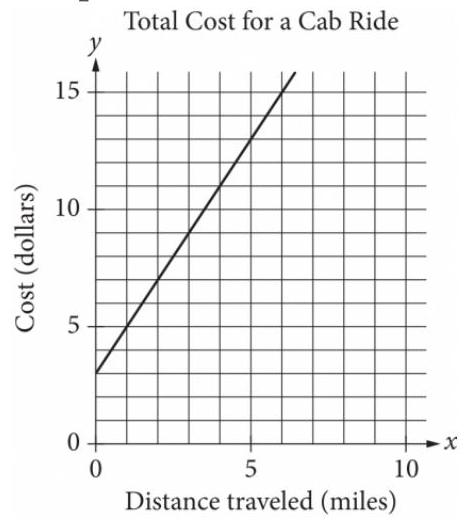
\includegraphics[width=0.70\linewidth]{images/2025_06_15_1eff2981bb1cf12f04f1g-18}
\end{center}

According to the graph, what is the cost for each additional mile traveled, in dollars, of a cab ride?
\begin{choices}
  \choice \$2.00
  \choice \$2.60
  \choice \$3.00
  \choice \$5.00
\end{choices}

\question[1]
A team of workers has been moving cargo off of a ship. The equation below models the approximate number of tons of cargo, $y$, that remains to be moved $x$ hours after the team started working.
\[y=120-25x\]
The graph of this equation in the $xy$-plane is a line. What is the best interpretation of the $x$-intercept in this context?
\begin{choices}
  \CorrectChoice The team will have moved all the cargo in about 4.8 hours.
  \choice The team has been moving about 4.8 tons of cargo per hour.
  \choice The team has been moving about 25 tons of cargo per hour.
  \choice The team started with 120 tons of cargo to move.
\end{choices}


\newpage


\question[1]
The function $F$ gives the temperature, in degrees Fahrenheit, that corresponds to a temperature of $x$ kelvins. If a temperature increased by 9.10 kelvins, by how much did the temperature increase, in degrees Fahrenheit?
\[F(x)=\frac{9}{5}(x-273.15)+32\]
\begin{choices}
  \CorrectChoice 16.38
  \choice 48.38
  \choice 475.29
  \choice 507.29
\end{choices}

\question[1]
In the given equation, $b$ is a constant. If the equation has no solution, what is the value of $b$?
\[(b-2)x=8\]
\begin{choices}
  \CorrectChoice 2
  \choice 4
  \choice 6
  \choice 10
\end{choices}

\question[1]
How many solutions does the equation $10(15x-9)=-15(6-10x)$ have?
\begin{choices}
  \choice Exactly one
  \choice Exactly two
  \CorrectChoice Infinitely many
  \choice Zero
\end{choices}

\newpage


\question[1]
\[
  \frac{4x}{5}=20
\]
In the equation above, what is the value of $x$?
\begin{choices}
  \CorrectChoice 25
  \choice 24
  \choice 16
  \choice 15
\end{choices}

\question[1]
\[3(kx+13)=\frac{48}{17}x+36\]
In the given equation, $k$ is a constant. The equation has no solution. What is the value of $k$?
\begin{solution}
$\frac{16}{17}$
\end{solution}

\question[1]
Which of the following is equivalent to $4x+6=12$?
\begin{choices}
  \choice $2x+4=6$
  \choice $x+3=3$
  \choice $3x+2=4$
  \CorrectChoice $2x+3=6$
\end{choices}



\newpage



\question[1]
One pound of grapes costs \$2. At this rate, how many dollars will $c$ pounds of grapes cost?
\begin{choices}
  \CorrectChoice $2c$
  \choice $2+c$
  \choice $\frac{2}{c}$
  \choice $\frac{c}{2}$
\end{choices}

\question[1]
A principal used a total of 25 flags that were either blue or yellow for field day. The principal used 20 blue flags. How many yellow flags were used?
\begin{choices}
  \CorrectChoice 5
  \choice 20
  \choice 25
  \choice 30
\end{choices}

\question[1]
\[8x=88\]
What value of $x$ is the solution to the given equation?
\begin{choices}
  \CorrectChoice 11
  \choice 80
  \choice 96
  \choice 704
\end{choices}




\newpage



\question[1]
A certain product costs a company \$65 to make. The product is sold by a salesperson who earns a commission that is equal to 20\% of the sales price of the product. The profit the company makes for each unit is equal to the sales price minus the combined cost of making the product and the commission. If the sales price of the product is \$100, which of the following equations gives the number of units, $u$, of the product the company sold to make a profit of \$6,840?
\begin{choices}
  \CorrectChoice $(100(1-0.2)-65)u=6,840$
  \choice $(100-65)(1-0.8)u=6,840$
  \choice $0.8(100)-65u=6,840$
  \choice $(0.2(100)+65)u=6,840$
\end{choices}

\question[1]
\[3a+4b=25\]
A shipping company charged a customer \$25 to ship some small boxes and some large boxes. The equation above represents the relationship between $a$, the number of small boxes, and $b$, the number of large boxes, the customer had shipped. If the customer had 3 small boxes shipped, how many large boxes were shipped?
\begin{choices}
  \choice 3
  \CorrectChoice 4
  \choice 5
  \choice 6
\end{choices}

\question[1]
What is the equation of the line that passes through the point $(0,5)$ and is parallel to the graph of $y=7x+4$ in the $xy$ plane?
\begin{choices}
  \choice $y=5x$
  \CorrectChoice $y=7x+5$
  \choice $y=7x$
  \choice $y=5x+7$
\end{choices}




\newpage



\question[1]
\[x+y=75\]
The equation above relates the number of minutes, $x$, Maria spends running each day and the number of minutes, $y$, she spends biking each day. In the equation, what does the number 75 represent?
\begin{choices}
  \choice The number of minutes spent running each day
  \choice The number of minutes spent biking each day
  \CorrectChoice The total number of minutes spent running and biking each day
  \choice The number of minutes spent biking for each minute spent running
\end{choices}


\question[1]
Line $t$ in the $xy$-plane has a slope of $-\frac{1}{3}$ and passes through the point $(9,10)$. Which equation defines line $t$?
\begin{choices}
  \choice $y=13x-\frac{1}{3}$
  \choice $y=9x+10$
  \choice $y=-\frac{x}{3}+10$
  \CorrectChoice $y=-\frac{x}{3}+13$
\end{choices}

\question[1]
A machine makes large boxes or small boxes, one at a time, for a total of 700 minutes each day. It takes the machine 10 minutes to make a large box or 5 minutes to make a small box. Which equation represents the possible number of large boxes, $x$, and small boxes, $y$, the machine can make each day?
\begin{choices}
  \choice $5x+10y=700$
  \CorrectChoice $10x+5y=700$
  \choice $(x+y)(10+5)=700$
  \choice $(10+x)(5+y)=700$
\end{choices}




\newpage



\question[1]
A total of 364 paper straws of equal length were used to construct two types of polygons: triangles and rectangles. The triangles and rectangles were constructed so that no two polygons had a common side. The equation $3x+4y=364$ represents this situation, where $x$ is the number of triangles constructed and $y$ is the number of rectangles constructed. What is the best interpretation of $(x,y)=(24,73)$ in this context?
\begin{choices}
  \CorrectChoice If 24 triangles were constructed, then 73 rectangles were constructed.
  \choice If 24 triangles were constructed, then 73 paper straws were used.
  \choice If 73 triangles were constructed, then 24 rectangles were constructed.
  \choice If 73 triangles were constructed, then 24 paper straws were used.
\end{choices}


\question[1]
The equation $y=0.1x$ models the relationship between the number of different pieces of music a certain pianist practices, $y$, during an $x$-minute practice session. How many pieces did the pianist practice if the session lasted 30 minutes?
\begin{choices}
  \choice 1
  \CorrectChoice 3
  \choice 10
  \choice 30
\end{choices}

\question[1]
In the $xy$-plane, line $k$ intersects the $y$-axis at the point $(0,-6)$ and passes through the point $(2,2)$. If the point $(20,w)$ lies on line $k$, what is the value of $w$?
\begin{solution}
74
\end{solution}

\question[1]
\phantom{\space}\\
\begin{center}
  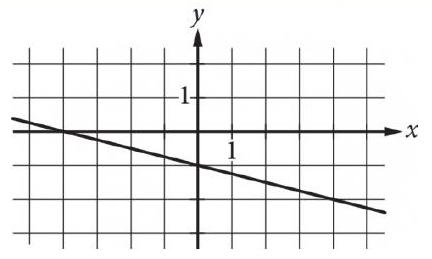
\includegraphics[width=0.90\linewidth]{images/2025_06_15_8c4b9d94a674ec08620fg-19}
\end{center}
Which of the following is an equation of the graph shown in the $xy$-plane above?
\begin{choices}
  \choice $y=-\frac{1}{4}x-1$
  \choice $y=-x-4$
  \choice $y=-x-\frac{1}{4}$
  \choice $y=-4x-1$
\end{choices}

\question[1]
An employee at a restaurant prepares sandwiches and salads. It takes the employee 1.5 minutes to prepare a sandwich and 1.9 minutes to prepare a salad. The employee spends a total of 46.1 minutes preparing $x$ sandwiches and $y$ salads. Which equation represents this situation?
\begin{choices}
  \choice $1.9x+1.5y=46.1$
  \CorrectChoice $1.5x+1.9y=46.1$
  \choice $x+y=46.1$
  \choice $30.7x+24.3y=46.1$
\end{choices}




\newpage



\question[1]
A local transit company sells a monthly pass for \$95 that allows an unlimited number of trips of any length.
What is the minimum number of trips per month for which a monthly pass could cost less than purchasing individual tickets for trips?
Individual tickets cost \$1.50, \$2.50, or \$3.50, depending on the length of the trip.
\begin{solution}
28
\end{solution}

\question[1]
A bakery sells trays of cookies. Each tray contains at least 50 cookies but no more than 60. Which of the following could be the total number of cookies on 4 trays of cookies?
\begin{choices}
  \choice 165
  \CorrectChoice 205
  \choice 245
  \choice 285
\end{choices}

\question[1]
  \[y<-4x+4\]
Which point $(x,y)$ is a solution to the given inequality in the $xy$-plane?
\begin{choices}
  \CorrectChoice $(-4,0)$
  \choice $(0,5)$
  \choice $(2,1)$
  \choice $(2,-1)$
\end{choices}




\newpage




\question[1]
A certain elephant weighs 200 pounds at birth and gains more than 2 but less than 3 pounds per day during its first year. Which of the following inequalities represents all possible weights $w$, in pounds, for the elephant 365 days after birth?
\begin{choices}
  \choice $400<w<600$
  \choice $565<w<930$
  \choice $730<w<1,095$
  \CorrectChoice $930<w<1,295$
\end{choices}

\question[1]
  $H=120p+60$\\
The Karvonen formula above shows the relationship between Alice's target heart rate $H$, in beats per minute (bpm), and the intensity level $p$ of different activities. When $p=0$, Alice has a resting heart rate. When $p=1$, Alice has her maximum heart rate. It is recommended that $p$ be between 0.5 and 0.85 for Alice when she trains. Which of the following inequalities describes Alice's target training heart rate?
\begin{choices}
  \CorrectChoice $120 \leq H \leq 162$
  \choice $102 \leq H \leq 120$
  \choice $60 \leq H \leq 162$
  \choice $60 \leq H \leq 102$
\end{choices}





\newpage



\question[1]
A petting zoo sells two types of tickets. The standard ticket, for admission only, costs \$5. The premium ticket, which includes admission and food to give to the animals, costs \$12. One Saturday, the petting zoo sold a total of 250 tickets and collected a total of \$2,300 from ticket sales. Which of the following systems of equations can be used to find the number of standard tickets, $s$, and premium tickets, $p$, sold on that Saturday?
\begin{choices}
  \CorrectChoice $\left\{\begin{aligned} s+p&=250 \\ 5s+12p&=2,300 \end{aligned}\right.$
  \choice $\left\{\begin{aligned} s+p&=250 \\ 12s+5p&=2,300 \end{aligned}\right.$
  \choice $\left\{\begin{aligned} 5s+12p&=250 \\ s+p&=2,300 \end{aligned}\right.$
  \choice $\left\{\begin{aligned} 12s+5p&=250 \\ s+p&=2,300 \end{aligned}\right.$
\end{choices}

\question[1]
\[\begin{gathered}
  x+y=18 \\
  5y=x
  \end{gathered}\]
What is the solution $(x,y)$ to the given system of equations?
\begin{choices}
  \CorrectChoice $(15,3)$
  \choice $(16,2)$
  \choice $(17,1)$
  \choice $(18,0)$
\end{choices}


\question[1]
\[\begin{gathered}
  x=10 \\
  y=x+21
  \end{gathered}\]
The solution to the given system of equations is $(x,y)$. What is the value of $y$?
\begin{choices}
  \choice 2.1
  \choice 10
  \choice 21
  \CorrectChoice 31
\end{choices}


\newpage



\question[1]
\[\begin{gathered}
  y=2x+10 \\
  y=2x-1
  \end{gathered}\]
At how many points do the graphs of the given equations intersect in the $xy$-plane?
\begin{choices}
  \CorrectChoice Zero
  \choice Exactly one
  \choice Exactly two
  \choice Infinitely many
\end{choices}

\question[1]
\[\begin{gathered}
  4x-6y=10y+2 \\
  ty=\frac{1}{2}+2x
  \end{gathered}\]
In the given system of equations, $t$ is a constant. If the system has no solution, what is the value of $t$?
\begin{solution}
8
\end{solution}


\question[1]
\[\begin{gathered}
  y=-\frac{1}{9}x \\
  y=\frac{1}{2}x
  \end{gathered}\]
The solution to the given system of equations is $(x,y)$. What is the value of $x$?
\begin{choices}
  \choice -9
  \choice -7
  \CorrectChoice 0
  \choice 2
\end{choices}

\newpage



\question[1]
\[\begin{aligned}
  & x+5y=5 \\
  & 2x-y=-4
  \end{aligned}\]
Which of the following graphs in the $xy$-plane could be used to solve the system of equations above?
\begin{choices}
  \choice 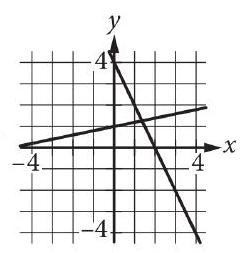
\includegraphics[width=0.70\linewidth]{images/2025_06_15_7d5ca6a095740ea44a32g-15}
  \choice 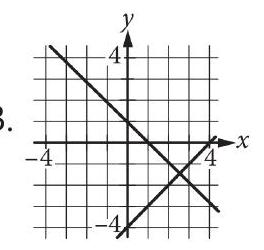
\includegraphics[width=0.70\linewidth]{images/2025_06_15_7d5ca6a095740ea44a32g-15(1)}
  \choice 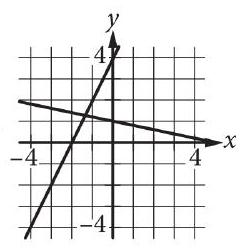
\includegraphics[width=0.70\linewidth]{images/2025_06_15_7d5ca6a095740ea44a32g-15(3)}
  \choice 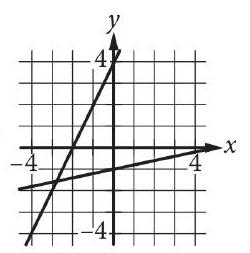
\includegraphics[width=0.70\linewidth]{images/2025_06_15_7d5ca6a095740ea44a32g-15(2)}
\end{choices}


\newpage


\question[1]
A bus traveled on the highway and on local roads to complete a trip of 160 miles. The trip took 4 hours. The bus traveled at an average speed of 55 miles per hour (mph) on the highway and an average speed of 25 mph on local roads. If $x$ is the time, in hours, the bus traveled on the highway and $y$ is the time, in hours, it traveled on local roads, which system of equations represents this situation?
\begin{choices}
  \choice $\begin{aligned} 55x+25y&=4 \\ x+y&=160 \end{aligned}$
  \CorrectChoice $\begin{aligned} 55x+25y&=160 \\ x+y&=4 \end{aligned}$
  \choice $\begin{aligned} 25x+55y&=4 \\ x+y&=160 \end{aligned}$
  \choice $\begin{aligned} 25x+55y&=160 \\ x+y&=4 \end{aligned}$
\end{choices}

\question[1]
\[\begin{gathered}
  y=2x+3 \\
  x=1
  \end{gathered}\]
What is the solution $(x,y)$ to the given system of equations?
\begin{choices}
  \choice $(1,2)$
  \CorrectChoice $(1,5)$
  \choice $(2,3)$
  \choice $(2,7)$
\end{choices}

\newpage


\question[1]
A system of two linear equations is graphed in the $xy$-plane below.

\begin{center}
  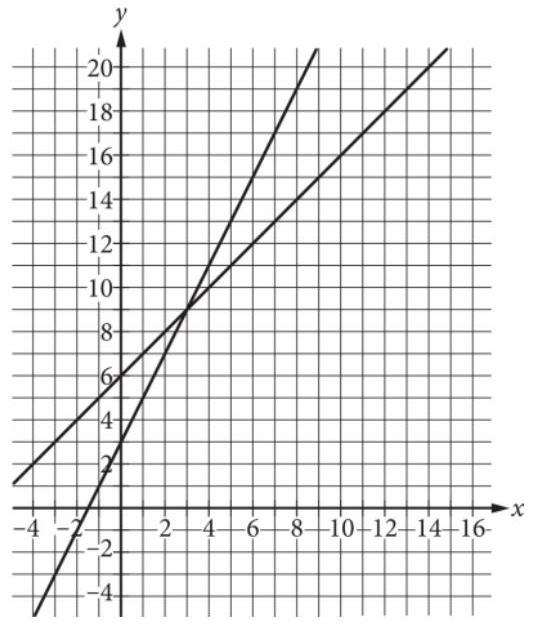
\includegraphics[width=0.90\linewidth]{images/2025_06_15_7d5ca6a095740ea44a32g-20}
\end{center}

Which of the following points is the solution to the system of equations?
\begin{choices}
  \choice $(3,9)$
  \choice $(6,15)$
  \choice $(8,10)$
  \choice $(12,18)$
\end{choices}

\endgradingrange{sat-drill-05}